\documentclass[12pt]{article}
\usepackage{url,graphicx,tabularx,array,geometry, extramarks, fancyhdr, lastpage,amsthm, amsmath, amssymb, mathtools}
\setlength{\parskip}{1ex} %--skip lines between paragraphs
%\setlength{\parindent}{10pt} %--don't indent paragraphs
\setlength\parindent{24pt}

%-- Commands for header
\renewcommand{\title}[1]{\textbf{#1}\\}
\renewcommand{\line}{\begin{tabularx}{\textwidth}{X>{\raggedleft}X}\hline\\\end{tabularx}\\[-0.5cm]}
\newcommand{\leftright}[2]{\begin{tabularx}{\textwidth}{X>{\raggedleft}X}#1%
& #2\\\end{tabularx}\\[-0.5cm]}

% Set up the header and footer
\pagestyle{fancy}
\lhead{\hmwkAuthorName} % Top left header
%\chead{\hmwkClass\  \hmwkTitle} % Top center head
\rhead{\hmwkDueDate} % Top right header
\lfoot{\lastxmark} % Bottom left footer
\cfoot{} % Bottom center footer
\rfoot{Page\ \thepage\ of\ \protect\pageref{LastPage}} % Bottom right footer
\renewcommand\headrulewidth{0.4pt} % Size of the header rule
\renewcommand\footrulewidth{0.4pt} % Size of the footer rule

\newcommand{\hmwkTitle}{HW\ \#4} % Assignment title
\newcommand{\hmwkDueDate}{\ May\ 14,\ 2014} % Due date
\newcommand{\hmwkClass}{STAT\ 243} % Course/class
%\newcommand{\hmwkClassTime}{10:30am} % Class/lecture time%
%\newcommand{\hmwkClassInstructor}{Jones} % Teacher/lecturer%
\newcommand{\hmwkAuthorName}{Angela Andrews, Nicholas Lytal} % Your name%leftright{\today}{Angela Andrews} %-- left and right positions in the header

\newcommand{\partdiv}[2]{\frac{\partial #1}{\partial #2}}
\newcommand{\logpart}[1]{\frac{\partial l_R}{\partial #1}}
\newcommand{\logpartsq}[1]{\frac{\partial^2 l_R}{\partial #1}}
\newcommand{\Pmat}{A(A'VA)^{-1}A'}
\newcommand{\partp}{\frac{\partial P}{\partial \theta_i}}
\newcommand{\ppartial}{-P\partdiv{V}{\theta_i}P}
\newcommand{\lo}{\mathrm{log}}
\newcommand{\tone}{\theta_1}
\newcommand{\ttwo}{\theta_2}
\newcommand{\ex}{\mathrm{exp}}
%\linespread{2} %-- Uncomment for Double Space
\begin{document}

\center{\title{STAT 243 HW\#4}}

\begin{description}

%%%%%%%%
% Problem 1  %
%%%%%%%%

\item[1.] We use the Monte Carlo method to evaluate each of the following integrals:
\begin{description}
\item[a.] \[\int_0^1 x^2 dx\]
The exact integral is calculated, for comparison, as:
\[\int_0^1 x^2 dx = \left. \frac{x^3}{3} \right|_0^1 = \frac{1}{3} \approx .333\bar{3} \]
Here, we let $f(x) = \frac{1}{1-0}$, a Uniform(0,1) distribution, and we let $h(x) = x^2$. We take 1,000,000 samples from a Uniform(0,1), and using the Monte Carlo method we obtain an estimate of the evaluated integral as .333328, or equivalenty $\frac{1}{3}$. Thus, we see that the Monte Carlo Method estimated the integral accurately. 

\item[b.] \[\int_0^1 \int^2_{-2} x^2 \mathrm{cos}(xy) \ \ dx dy\]

We solve the exact integral using computational tools for comparison purposes, and obtain

\[\int_0^1 \int^2_{-2} x^2 \mathrm{cos}(xy) \ \ dx dy \approx 3.48318\]

Here, since we have two variables, instead of having $f(x)$ and $h(x)$, we will instead have $f(x,y)$ and $h(x,y)$. Here, we let $f(x,y) = \frac{1}{4}$ and we let $h(x,y) = 4x^2\mathrm{cos}(xy)$. Thus, we see that $\int_0^1 \int_{-1}^2 \frac{1}{4} = 1$, which satisfies our condition for $f(x,y)$. We sample from a Uniform(-2,2) for x and from a Uniform(0,1) for y, each 1,000,000 times, and we plug these values into our function $h(x,y)$. Thus, taking 1,000,000 samples from the two Uniform distribution and using the Monte Carlo method, we obtain an estimate of the evaluated integral of 3.480481. Thus, we see that the Monte Carlo method produced an accurate estimate of the integral. 

\item[c.] \[\int_0^\infty \frac{3}{4} x^4 e^{-\frac{x^3}{4}} dx\]

We solve the exact integral for comparison. Using computational tools we obtain:
\[\int_0^\infty \frac{3}{4} e^{-\frac{x^3}{4}} dx = 2 \sqrt[3]{2} \Gamma \left( \frac{5}{3} \right) \approx 2.27478 \]

Here, we see that the integral is over a very large range (0 to $\infty$), compared to the other integrals that we have evaluated. As a result, we do not expect to obtain as accurate results for evaluating the integral as we did in parts a and b. Thus, here we estimate the integral 100 times using 1,000,000 samples and the Monte Carlo method, and plot the density to see the value that the estimates center themselves around. For this integral, we let $f(x)$ and $h(x)$ be defined as:

\[f(x) = \frac{\frac{1}{4}^5}{\Gamma(5)} \cdot x^4 \mathrm{exp}\left(-\frac{x}{4} \right) \sim \mathrm{Gamma}(5, 0.25)\]

\[h(x) = \frac{3}{4} \cdot \frac{\Gamma(5)}{\frac{1}{4}^5} \cdot \mathrm{exp} \left( \frac{x}{4} - \frac{x^3}{4}\right)\]

Thus, we take 1,000,000 samples of x from $x \sim \Gamma(5, 0.25)$ and plug these into $h(x)$ to be used in the formula for estimating the integral. Repeating this process 1000 times, we obtain the following density plot of evaluated integral estimates. The vertical red line represents the maximum of the density, which occurs at the value 2.25775. Here we see that the Monte Carlo method did not approximate the integral as accurately as previous integrals that we approximated (see parts a and b). However, this is expected since we have such a large range that we are integrating over (to infinity). In previous problems, we were integrating over a finite interval of numbers, allowing for more accurate approximation. 

\[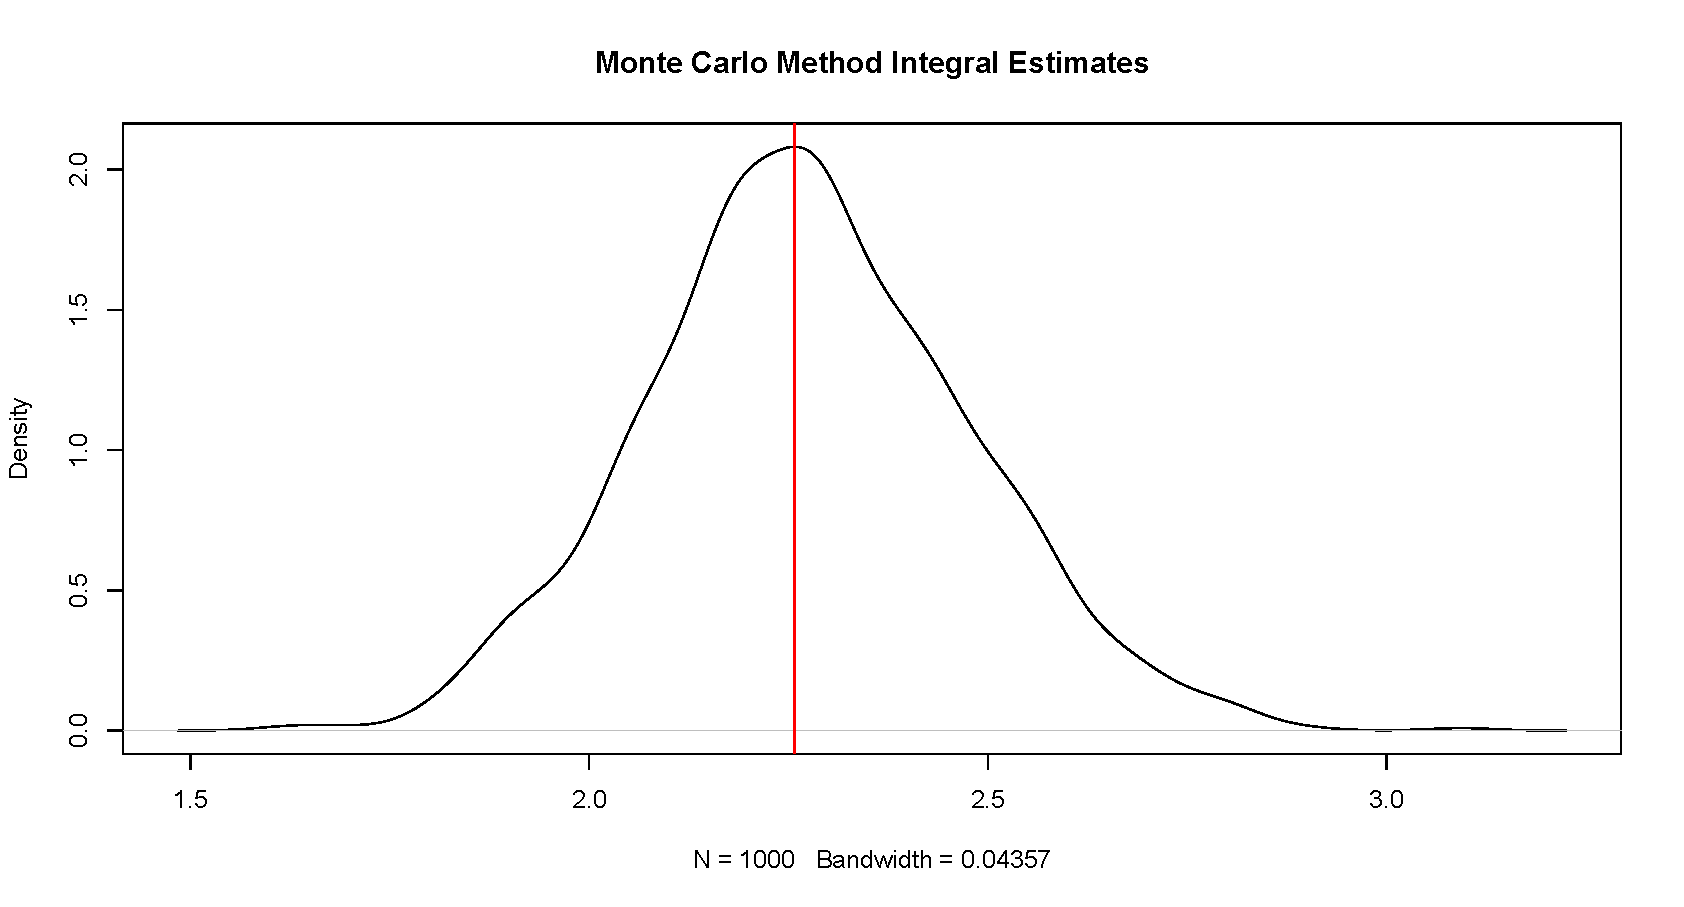
\includegraphics[scale = 0.50]{STA243HW4Plot1}\]
\end{description}

%%%%%%%%
% Problem 2  %
%%%%%%%%
\item[2.] We let
\[I = \frac{1}{\sqrt{2\pi}} \int_1^2 e^{-\frac{x^2}{2}}dx \]
and estimate $I$ using importance sampling. We take $g$ to be $N(1.5, \nu^2)$ with $\nu = 0.1$ and 10. 


Given that $g(x) \sim N(1.5, \nu^2)$, we must find $h(x)$ such that
\[\int_{-\infty}^{\infty} h(x)\cdot \frac{f(x)}{g(x)} \cdot  \frac{1}{\sqrt{2\pi \nu^2}} \ex\left\{ -\frac{(x - 1.5)^2}{2 \nu^2}\right\}=\frac{1}{\sqrt{2\pi}} \int_1^2 e^{-\frac{x^2}{2}}dx \]

\[\int_{-\infty}^{\infty} h(x)\cdot \frac{f(x)}{\frac{1}{\sqrt{2\pi \nu^2}} \ex\left\{ -\frac{(x - 1.5)^2}{2 \nu^2}\right\}} \cdot  \frac{1}{\sqrt{2\pi \nu^2}} \ex\left\{ -\frac{(x - 1.5)^2}{2 \nu^2}\right\}=\frac{1}{\sqrt{2\pi}} \int_1^2 e^{-\frac{x^2}{2}}dx \]

Thus, we can easily see that we can let $h(x)$ be the indicator function as follows:

\[ h(x) = I_{\{1 < x < 2\}} = \left\{ 
\begin{array}{l l}
1 & \quad \text{if } 1 < x < 2\\
0 & \quad \text{otherwise}
\end{array} \right.\]

and we can let $f(x) \sim N(0, 1)$, the standard normal distribution. With $f(x)$ and $h(x)$ defined as these, we have:

\[\int_{-\infty}^{\infty} I_{\{1 < x < 2\}}\cdot \frac{\frac{1}{\sqrt{2\pi} \ex \left \{ -\frac{x^2}{2}\right\}}}{\frac{1}{\sqrt{2\pi \nu^2}} \ex\left\{ -\frac{(x - 1.5)^2}{2 \nu^2}\right\}} \cdot  \frac{1}{\sqrt{2\pi \nu^2}} \ex\left\{ -\frac{(x - 1.5)^2}{2 \nu^2}\right\}=\frac{1}{\sqrt{2\pi}} \int_1^2 e^{-\frac{x^2}{2}}dx\]

Now that we have defined $h(x)$ and $f(x)$, we carry out the Importance Sampling algorithm as follows:
\begin{description}
\item[1.] We generate $\tilde{x}_1, \dots, \tilde{x}_m$ iid from $g(\tilde{x}) \sim N(1.5, \nu^2)$.
\item[2.] We estimate $\mu = \int h(\tilde{x}) \cdot \frac{f(\tilde{x})}{g(\tilde{x})} \cdot g(\tilde{x}) dx$ by $\hat{\mu}_g = \frac{1}{m} \sum_{i=1}^m h(\tilde{x}_i | w(\tilde{x}_i))$ where $w(\tilde{x}_i)$ is the importance ration: $w(\tilde{x}_i) = \frac{f(\tilde{x})}{g(\tilde{x})}$
\end{description}

We first use a computational tool to solve the integral directly, for comparison purposes. In doing so, we obtain:

\[\frac{1}{\sqrt{2\pi}} \int_1^2 e^{-\frac{x^2}{2}}dx = \frac{1}{2} \left( \mathrm{erf}(\sqrt{2}) - \mathrm{erf}\left(\frac{1}{\sqrt{2}} \right) \right) \approx 0.135905\]

Where \textbf{erf} is the errror function. 
We carry out this process for $\nu = 0.1, 1, 10$, each with m = 1000000. From, these, we obtain the following estimates of the integral:
\[
\begin{tabular}{| r | c | c | c |}
\multicolumn{4}{c}{Integral Estimates} \\
\hline
$\nu$ & 0.1 & 1 & 10 \\
\hline
$\hat{\mu}_g$ & 0.03262997 & 0.1360167 & 0.01375336\\
\hline
\end{tabular}\]

Looking at these estimates, we see that $\nu = 1$ provided the best estimate for the integral. On the following pages, we plot histograms of the values which we averaged for each value of $\nu$, in order to determine if there are any extreme values. 

\[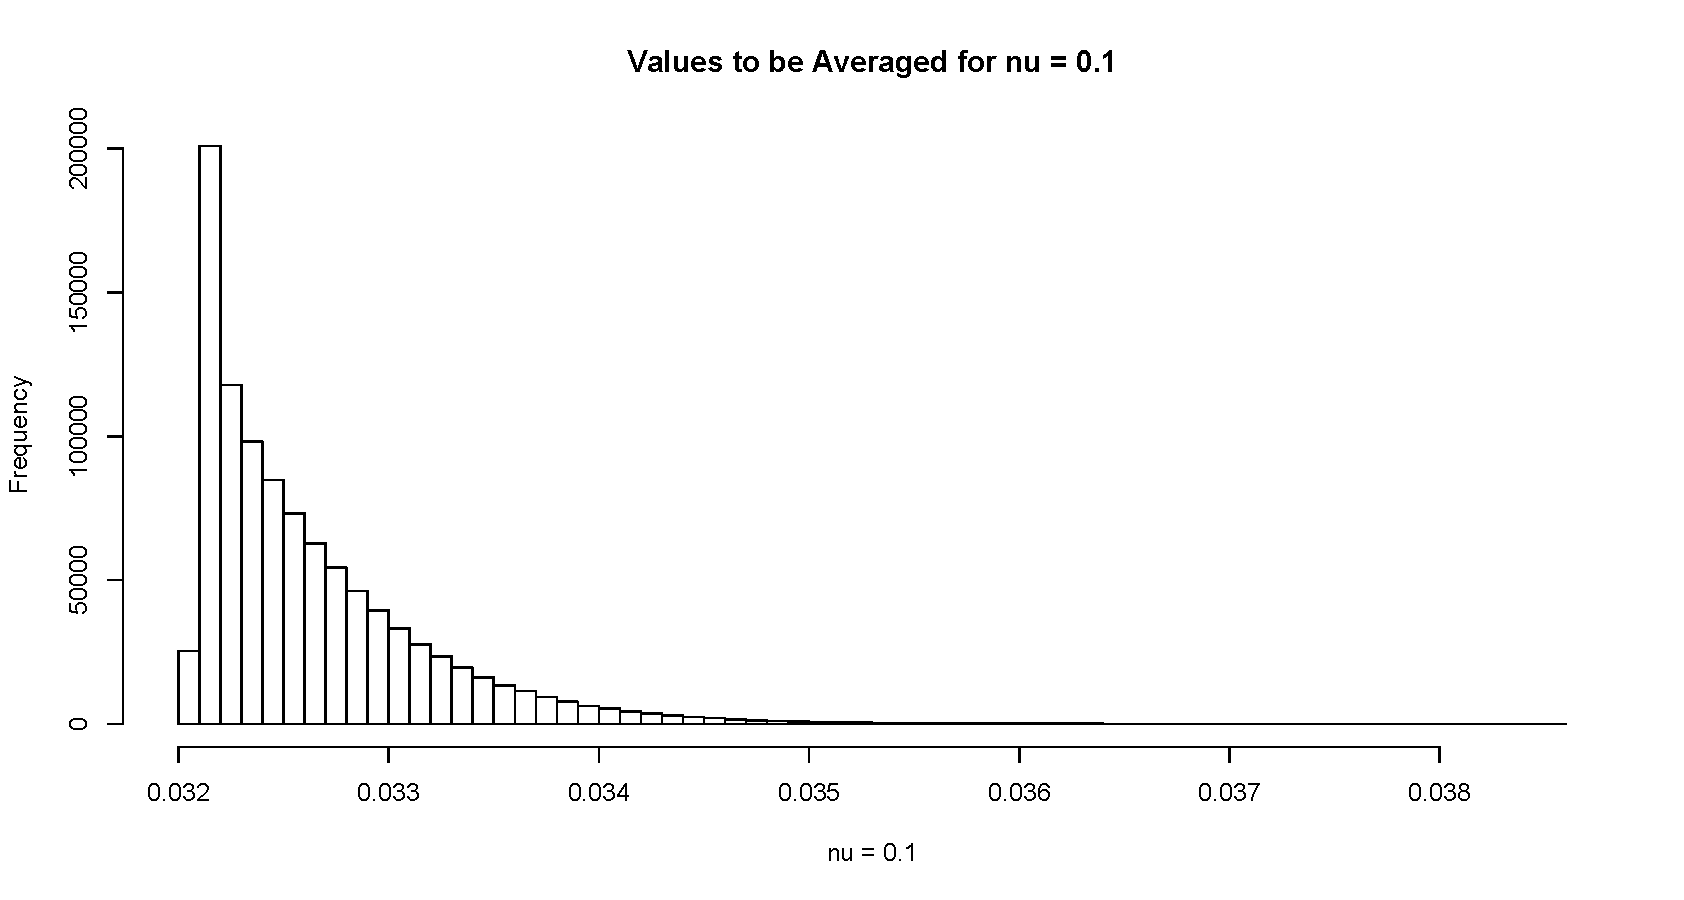
\includegraphics[scale = 0.50]{STA243HW4Plot2.pdf}\]

Looking at the histogram for $\nu = 0.1$, we see that it the values of $h(\tilde{x}_i | w(\tilde{x}_i))$ cover a range between 0.03210 and 0.03858. Thus, we see that none of the $\tilde{x}$ values generated from $g(\tilde{x})$ were outside of the range (1, 2), since we have no values that are equal to zero (and thus would have been rejected by the indicator function).  However, we also note that the majority of values of $h(\tilde{x}_i | w(\tilde{x}_i))$ appear to be between 0.032 and 0.035, which is a very small range, and is nowhere near what we know the true value of the integral to be. This is because, with such a small $\nu$, we are unable to explore the full space. Here,is also looks as if there are some extreme values on the upper end, as we see that the distribution is heavily skewed. 

\[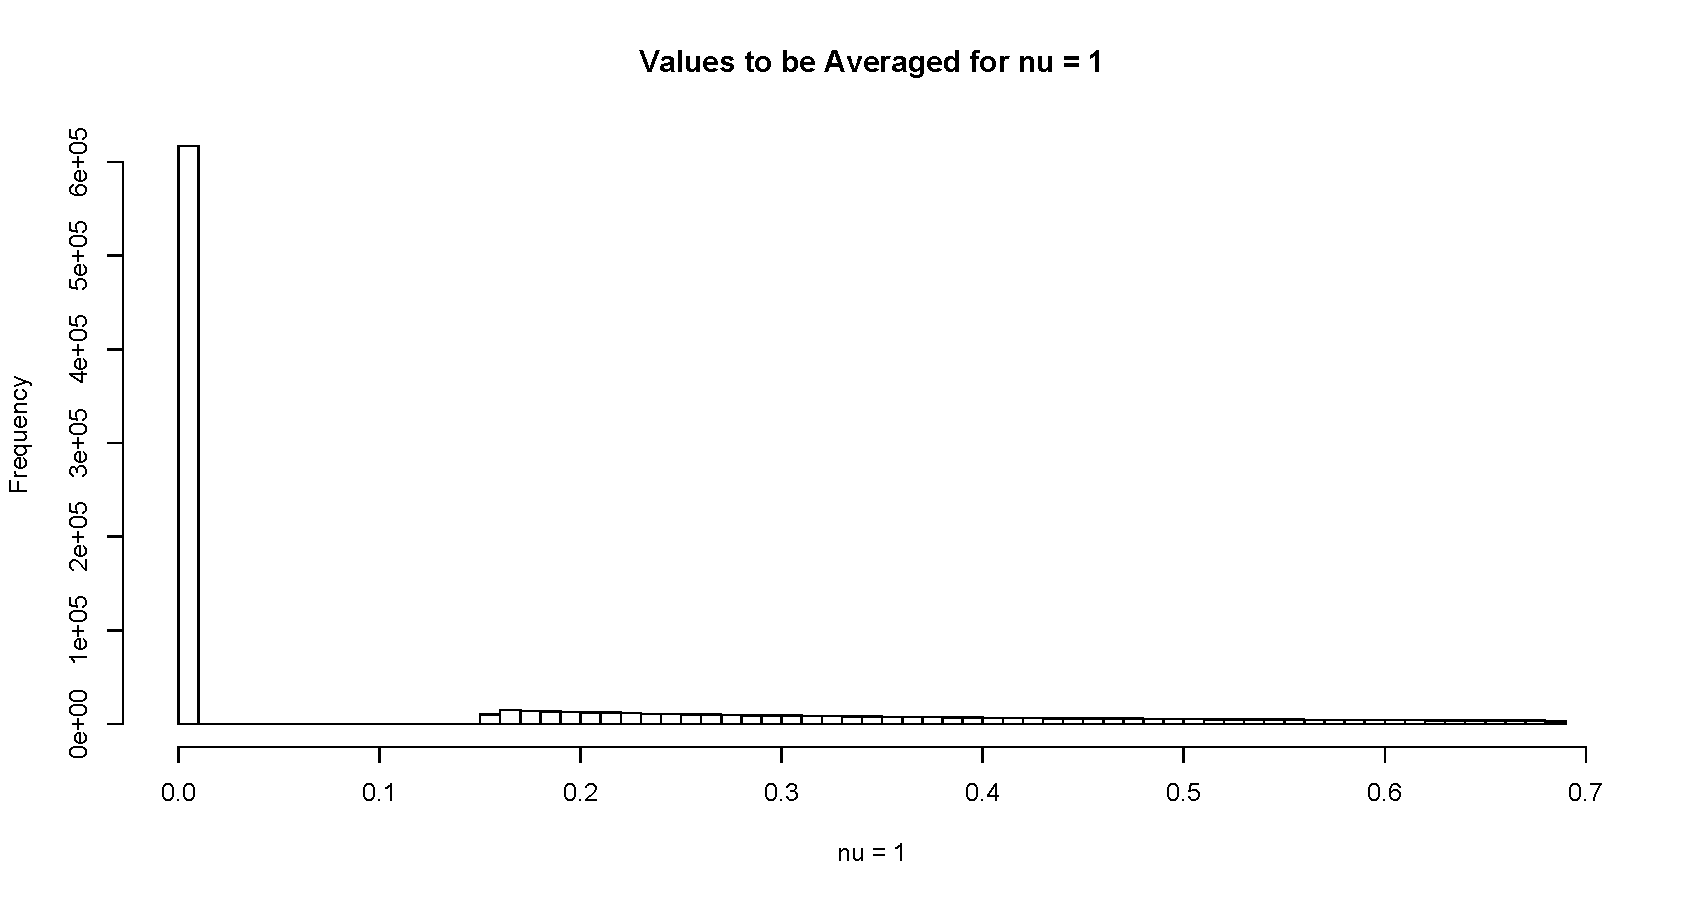
\includegraphics[scale = 0.50]{STA243HW4Plot3.pdf}\]

For $\nu = 1$, we see that our $h(\tilde{x}_i | w(\tilde{x}_i))$ values cover a much larger range. Here, we see that our values of $h(\tilde{x}_i | w(\tilde{x}_i))$ range from 0 to 0.6873. Here, we see that we have 617008 zeros, which means that there were 617008 or 61.7008\% of  $\tilde{x}$'s that were drawn outside of the range from 1 to 2. Here, we see that the $\nu$ was large enough to let us explore the entire range, yet not too large, as confirmed by our accurate estimate of the integral. This is to be expected, as in the original integral, we notice that we are simply integrating the standard normal distribution (and thus it has a variance of 1). Here, we let the variance of the underlying distirbution equl to 1, and we see that this leads to a very accurate estimate. 

\[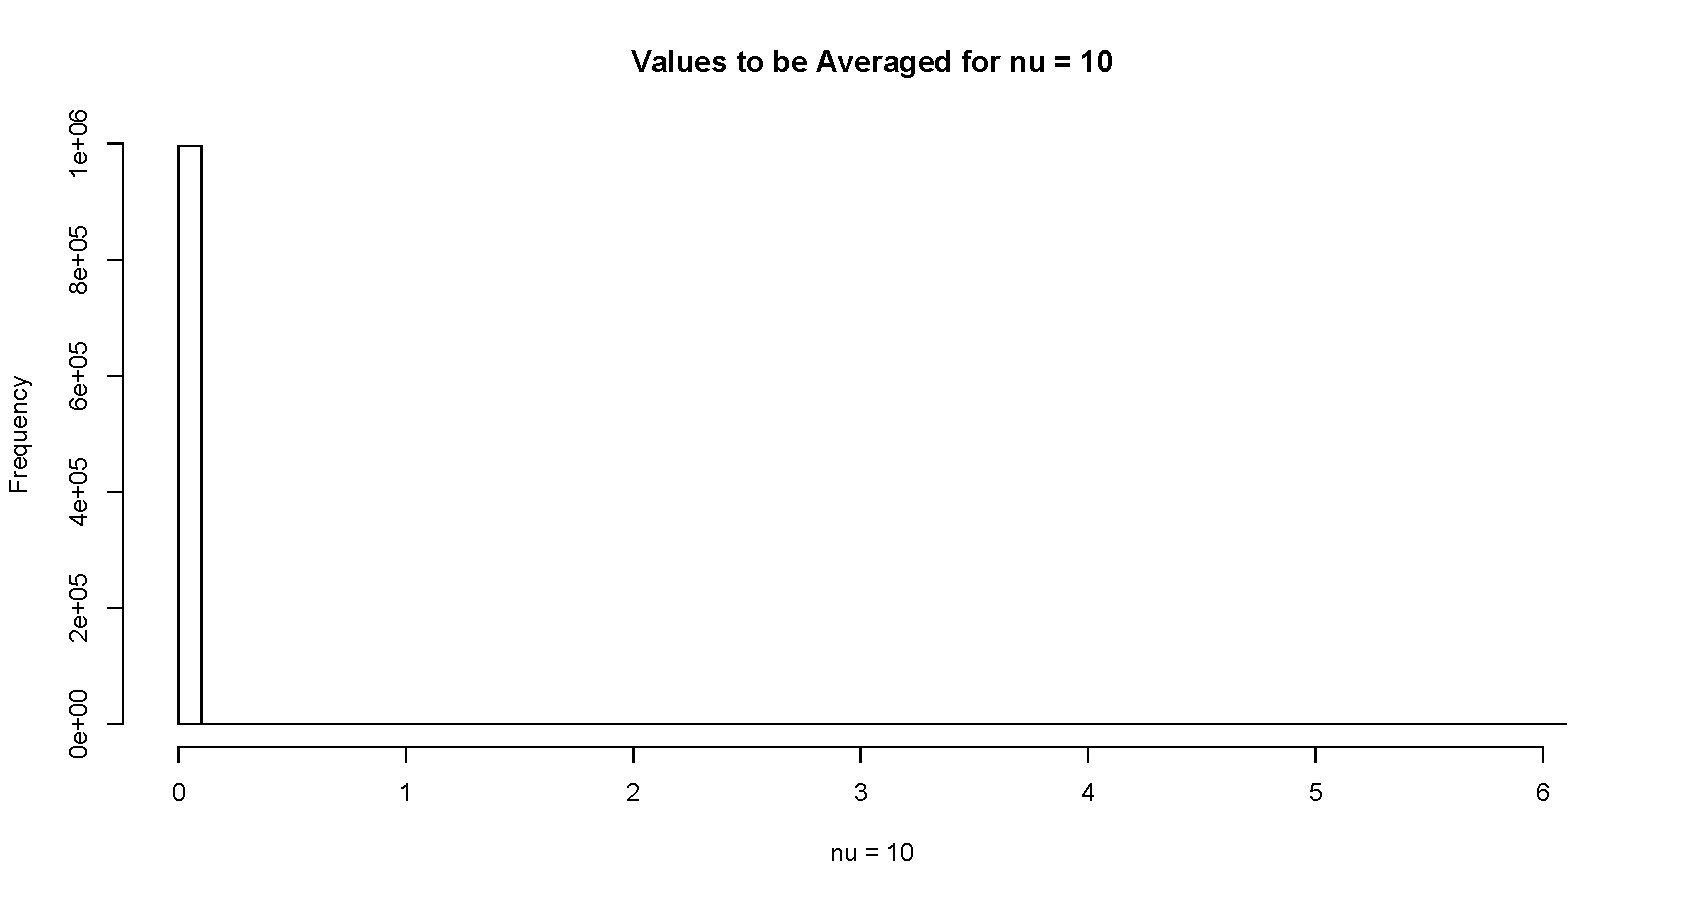
\includegraphics[scale = 0.50]{STA243HW4Plot4.pdf}\]

For $\nu = 10$, we see that almost all of the values of $\tilde{x}$ get pushed to zero, as they are almost all out of the range (1,2). Here, we have 995,961, or 99.5961\% of $\tilde{x}$'s that are sampled out of the (1,2) range and are thus made to be zero. This is expected, since the $\tilde{x}$'s were sampled from a N(1.5, 10) distibution, and thus with such a large variance, we would expect many of the values to fall outside of (1,2). Thus, here we see that the majority of values  of $h(\tilde{x}_i | w(\tilde{x}_i))$ are 0, as expected, with some extreme values on the top end, as we see that the range of the values of $h(\tilde{x}_i | w(\tilde{x}_i))$ extends all the way past 6. This pulls our estimate of the integral for $\nu = 10$ up, yet all of the zero's keep the estimate quite small. Again, this is expected since, with such a large in the underlying distribution, we explore a much larger space than we are actually interested in. 
%%%%%%%%
% Problem 3  %
%%%%%%%%

\item[3.] We will approximate the following integral using both the simple Monte Carlo integration and the control variate method:
\[I = \int_0^1 \frac{1}{1 + x} dx\]

\begin{description}
\item[a.]We let $h(x) = \frac{1}{1+x}$ and $U_1, \dots U_n$ be iid Unif[0,1]. We estimate $\hat{I}_{MC} = \frac{1}{n} \sum_{i = 1}^n h(U_i)$ with n = 1500 in R and obtain an estimate of $\hat{I}_{MC} = 0.6941916$. We note that the tru value for $I$ is known to be $I = \mathrm{ln}(2) = 0.6931472$, thus we see that our estimate for $I$ is accurate. 
\item[b.] Next, we introduct $c(x) = 1 + x$ as a control variate, and we estimate $i$ with:
\[\hat{I}_{CV} = \frac{1}{n} \sum_{i = 1}^n h(U_i) - b \left[ \frac{1}{n} \sum_{i = 1}^n c(U_i) - E\{c(U)\} \right]\]

In order to carry out this estimation, we must first find the optimal value of b to plug into the expression. From class, we know that the optimal value of b will minimize the variance of the estimator, $\hat{I}_{CV}$. Based on the derivations from class, we have that the optimal value of b which will minimize the variance of  $\hat{I}_{CV}$ is equal to:
\[b_{OPT} = \frac{\mathrm{cov}(\hat{I}_{CV}, \hat{\theta}_{MC})}{\mathrm{var}(\hat{\theta}_{MC})} = \frac{\mathrm{cov}(h(\tilde{x}), c(\tilde{U}))}{\mathrm{var}(c(\tilde{U}))} \]

where $\hat{\theta}_{MC} = \frac{1}{n} \sum_{i = 1}^n c(U_i)$.\\

Recall from part a that $h(x)  = \frac{1}{1 + x}$ and E[h(x)] = ln 2. What is left is to find E[c(U)] and cov(h(x), c(U)). Recall that $c(x) = 1 + x$ and since we are on the range of (0,1), we have that the expected value of c(x) is equal to 1.5. Thus, to find our optimal b, we first draw 1500 x's from $x \sim \mathrm{Unif}(0, 1)$, then plug these x's into $h(x) = \frac{1}{1 + x}$ and $c(x) = 1 + x$. We then estimate the covariance between these generated $h(x)$ and $c(x)$'s, and the variance of $c(x)$. In doing so, we obtain the following estimate of b: $b_{OPT} = -0.4747049$. 
\item[c.] We estimate the variances of $\hat{I}_{MC}$ and $\hat{I}_{CV}$ by taking 1,000,000 samples from each in R and obtain:
 \[\mathrm{var}(\hat{I}_{MC}) = 1.274619^{e-05}\] 
\[\mathrm{var}(\hat{I}_{CV}) = 4.002654e^{-07}\]
Thus, we see that the variance of $\hat{I}_{CV}$ is much smaller than the variance of $\hat{I}_{MC}$, as we would have hoped.  
\item[d.] Although we have already designed an estimator, $\hat{I}_{CV}$, which is much more efficient than our original estimator, $\hat{I}_{MC}$, it is still possible to design a new estimator for $I$ that would have a smaller variance that $\hat{I}_{CV}$. To do so, we would simply add another control variate, so that instead of just one control variate ($c(x) = 1 + x)$, we would have two control variates and thus estimate two b's. Thus, our estimate would be obtained by finding $b_1^*$ and $b_2^*$ that minimize the variance of the following function:
\[\hat{I}_{CV} = \hat{I}_{MC} - b_1(\hat{\theta}_{1MC} - \theta_1) - b_2(\hat{\theta}_{2MC} - \theta_2)\]

where $\hat{\theta}_{1MC} = \frac{1}{n} \sum_{i = 1}^n c_1(x_i)$ and $\hat{\theta}_{2MC} = \frac{1}{n} \sum_{i = 1}^n c_2(x_i)$, and $c_1(x_i)$ is the first control variate, and $c_2(x_i)$ is the second control variate. You could theoretically keep adding control variates in this fashion, until the variance reduction factor no longer reduces (adding addition control variates no longer minimizes the variance), or the changes in the variance reduction factor is arbitrary. The variance reduction factor is defined as:
\[\text{variance reduction factor} = \frac{\mathrm{var} (\hat{I}_{CV}^{OPT})}{\mathrm{var}(\hat{I}_{MC}^{OPT})} = 1 - \rho^2\]
where $\rho$ is the correlation coefficient between $h(\tilde{x})$ and $c(\tilde{x})$. However; in general, adding more control variates results equations that are both computationally and analytically difficult to solve, and thus at most only one or two control variates are generally used in practice.  
\end{description}


%%%%%%%%
% Problem 4  %
%%%%%%%%

\item[4.] We consider a common application in statistics: three different treatments are to be compared by applying them to a randomly selected experimental units. However; instead of the usualy assumption associated with $e_{ij}$ in the typical analysis of variance methods of comparison, we assume that the $e_{ij}$  have independent and identical double exponential distributions centered on zero.
\begin{itemize}
\item[a.]
\item[b.]
\end{itemize}


%%%%%%%%
% Problem 5  %
%%%%%%%%

\item[5.] We consider the zero-inflated Poisson( ZIP) model, in which random data $X_1, \dots, X_n$ are assumed to be of the form $X_i = R_iY_i$, where $Y_i$'s have a Poisson($\lambda$) distribution and the $R_i$'s have a Bernoulli($p$) distribution, all independent of each other. Given an outcome $x = (x_1, \dots, x_n)$, the objective is to estimate both $\lambda$ and $p$. We consider the following hierarchical Bayes model:
\begin{itemize}
\item $p \sim$ Uniform(0,1) (prior for $p$)
\item $(\lambda | p) \sim$ Gamma$(a, b)$ (prior for $\lambda$)
\item $(r_i | p, \lambda) \sim$ Bernoulli($p$) independently (from the model above)
\item $(x_i | r, \lambda, p) \sim$ Poisson($\lambda r_i$) independently (from the model above)
\end{itemize}
where $a$ and $b$ are known parameters, and $r = (r_1, \dots, r_n)$. It follows that:
\[f(x, r, \lambda, p) = \frac{b^a\lambda^{a-1}e^{-b\lambda}}{\Gamma(a)}\prod^n_{i = 1} \frac{e^{-\lambda r_i} (\lambda r_i)^{x_i}}{x_i!} p^{r_i} (1 - p)^{1 - r_i}\]

We wish to sample from the posterior pdf $f(\lambda, p, r | x)$ using the Gibbs sampler.\
\begin{description}
\item[a.]
\item[b.]
\item[c.]
\end{description}

%%%%%%%%
% Problem 6  %
%%%%%%%%

\item[6. ] The Independence - Metropolis - Hastings Algorithm is an importance-sampling version of MCMC. We draw the proposal from a fixed distribution $g$. Generally, $g$ is chosen to be an approximation to $f$. The acceptance probability becomes:
\[r(x, y) = min\left\{ \frac{f(y)}{f(x)} \cdot \frac{g(x)}{g(y)}, 1 \right\}\]

A random variable Z has an inverge Gaussian distribution it it has density

\[f(z) \propto z^{-3/2} \mathrm{exp}\left\{ -\theta_1z - \frac{\theta_2}{z} + 2\sqrt{\theta_1\theta_2} + \lo \sqrt{2\theta_2}\right\}, \ \ z >0\]

where $\theta_1 0$ and $\theta_2 >0$ are parameters. It can be shown that 
\[E(Z) = \sqrt{\frac{\theta_2}{\theta_1}} \ \ \ \ \mathrm{and} \ \ \ \ E\left(\frac{1}{Z} \right)= \sqrt{\frac{\theta_1}{\theta_2}} + \frac{1}{2\theta_2}\]

We let $\theta_1 = 1.5$ and $\theta_2 = 2$, and draw a sample of size 1,000 using the independence-Metropolis-Hastings algroithm. We use a Gamma distribution as the proposal density. Below is a density plot of the sample drawn using the Independence-Metropolis-Hastings algorithm with a Gamma distribution as the proposal density. 

\[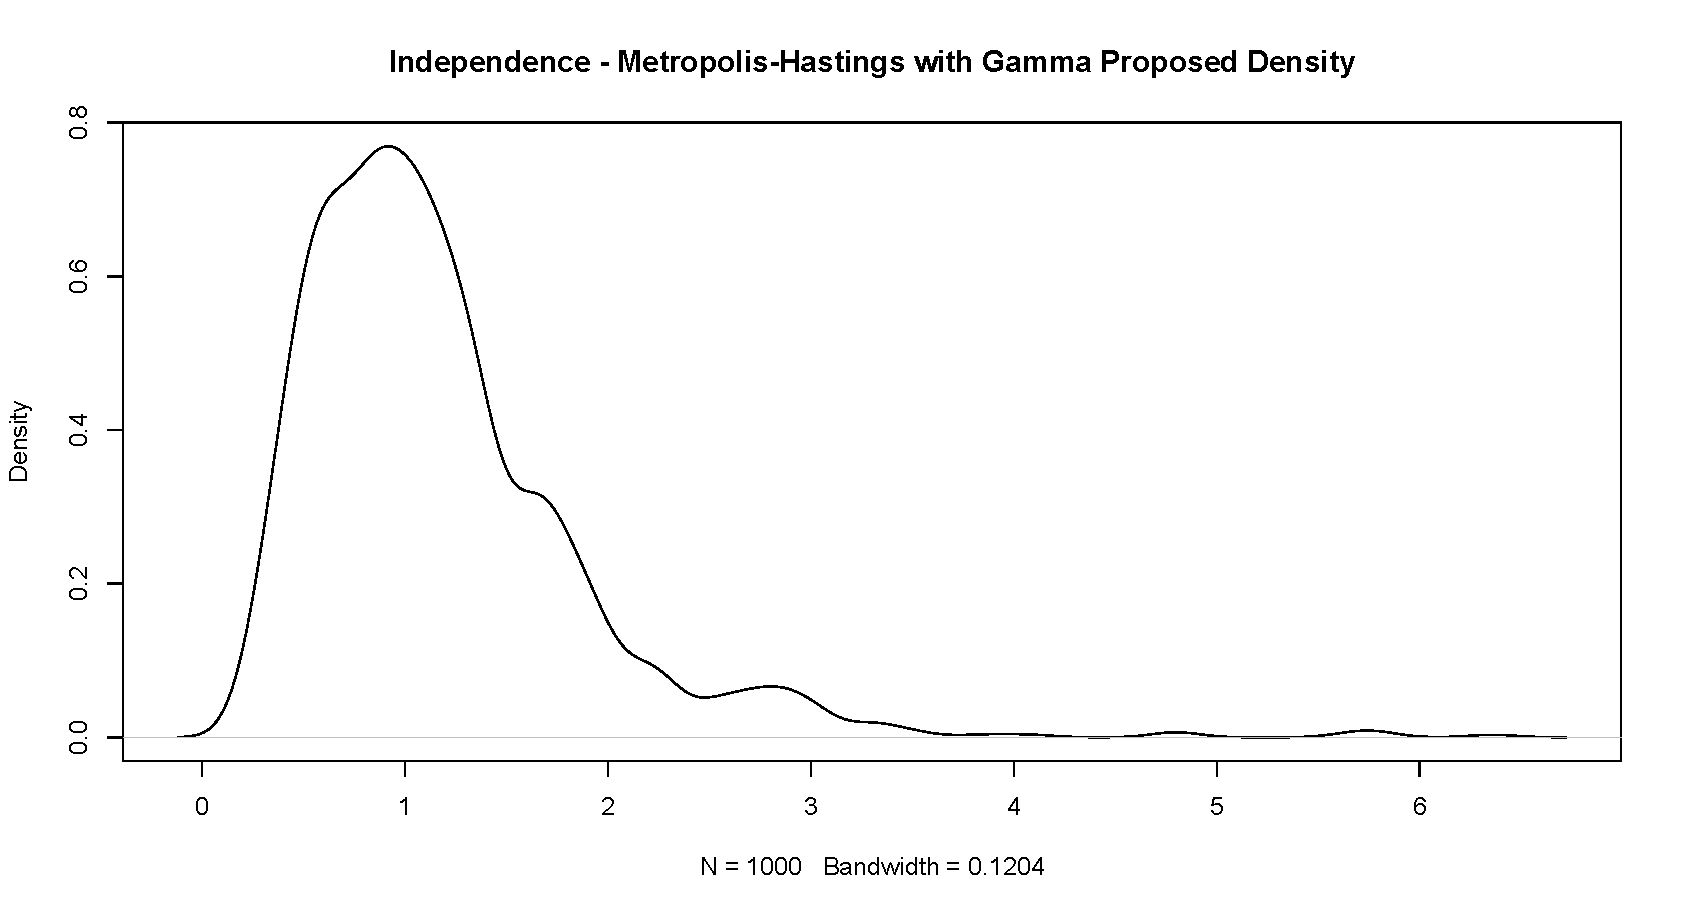
\includegraphics[scale = 0.50]{STA243HW4Q6Plot1.pdf}\]

To assess the accuracy of the Independence - Metropolis - Hastings algroithm, we compare the mean of $Z$ and $1/Z$ from the sample to the theoretical means. The theoretical means are derived below:

\[E[Z] = \sqrt{\frac{\theta_2}{\theta_1}} = \sqrt{\frac{2}{1.5}} \approx 1.154701\]
\[E\left[ \frac{1}{Z} \right] = \sqrt{\frac{\theta_1}{\theta_2}} + \frac{1}{2\theta_2} = \sqrt{\frac{1.5}{2}} + \frac{1}{2\cdot 2} \approx 1.116025\]

Our sample of n = 1,000,000 yields the following estimates of the means:

\[\hat{E}[Z] \approx 1.153933, \ \ \ \ \hat{E}\left[\frac{1}{Z}\right] \approx 1.116973\]

From this, we see that the Independence - Metropolis - Hastings algorithm performed pretty well, as the estimates based on our sample very, very similar to the theoretical values, to several decimal places. The remaining difference is likely due to the sample size, and we believe that the sample values will approach the theoretical values as n $\rightarrow \infty$. Thus, it appears that our sample is relatively accurate. \\

In addition to this $\theta_1$ and $\theta_2$, we try several different combinations of $\theta_1$ and $\theta_2$ in order to see if we can get accurate samples. For computational ease, we now let n = 1000 as opposed to n = 1000000 

\end{description}
\end{document}


